\chapter{Introduction}
\label{sec:intro}

On January 20th 1994 Canadians experienced an unexpected interruption to their television programming: The Canadian Telsat spacecraft Anik E1 and Anik E2 had experienced sudden failures of their gyroscopic guidance systems and had begun to tumble out of control. Later attributed to the phenomena of spacecraft charging, the Anik spacecraft had experienced electrostatic discharge of the gyroscope circuitry causing permanent damage to critical systems. Although engineers were able to restore the gyroscopes of Anik E1, the Anik E2 would never recover, representing a loss of several hundred million dollars \insertref{Leach1995}.

Spacecraft charging has been studied as a disparate field of research since the mid twentieth century, with fundamental theories describing the phenomena by Langmuir  


\parencite{Garrett1981} 




% \begin{equation}
%     \iint_D \diff x \diff y
%     =
%     \int_0^{2\pi} \int_0^t \rho \diff \rho \diff t
%     =
%     \frac{4}{3} \pi^3.
% \end{equation}

\section{Figures and Tables}

% Standalone with \input:
\begin{figure}[htbp]
    \centering
    \documentclass[tikz]{standalone}
\begin{document}
    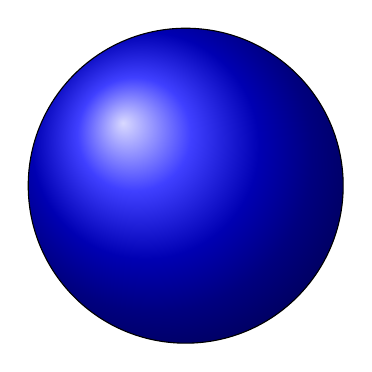
\begin{tikzpicture}
          \draw[shading = ball] (0, 0) circle (2);
    \end{tikzpicture}
\end{document}
    \caption[One ball]{One ball.}
\end{figure}

% Standalone with \includegraphics:
\begin{figure}[thbp]
    \centering
    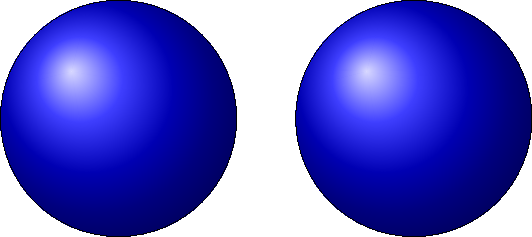
\includegraphics{balls}
    \caption[Two balls]{Two balls.}
\end{figure}

% Todonotes:
\begin{figure}[hbp]
    \centering
    \missingfigure{Three balls.}
    \caption[Three balls]{Three balls.}
\end{figure}

\kant[5-6] % Dummy text

% Booktabs:
% \begin{table}[htbp]
%     \centering
%     \begin{tabular}{@{}ll@{}}
%         \toprule
%         \textbf{Correct}               & \textbf{Incorrect}      \\
%         \midrule
%         \( \varphi \colon X \to Y \)   & \( \varphi : X \to Y \) \\[0.5ex]
%         \( \varphi(x) \coloneqq x^2 \) & \( \varphi(x) := x^2 \) \\
%         \bottomrule
%     \end{tabular}
%     \caption[Colons]{Proper colon usage.}
% \end{table}



\section{Outline}

The rest of the text is organised as follows:
\begin{description}
    \item[\cref{sec:theory}]
    is second to none, with the notable exception of \cref{sec:intro}.
    The main tool introduced here is the employment of unintelligible sentences.

    \item[\cref{sec:methods}]
    asserts the basic properties of being the third chapter of a text.
    This section reveals the shocking truth of filler content.

    \item[\cref{sec:results}]
    demonstrates how easily one can get to four chapters by simply using the \texttt{kantlipsum} package to generate dummy words.
    
    \item[\cref{sec:discussion}]
    demonstrates how easily one can get to four chapters by simply using the \texttt{kantlipsum} package to generate dummy words.

    \item[\cref{sec:first-app}]
    features additional material for the specially interested.

    \item[\cref{sec:second-app}]
    consists of results best relegated to the back of the document,
    ensuring that nobody will ever read it.
\end{description}